
\section{Psychometrics}
In the animated 1937 classic \textit{Clock Cleaners}, Mickey Mouse, Donald Duck, and Goofy are working as janitors in a clock tower. As usual, Goofy is dimwitted and carefree, Donald Duck gets fits of anger, and Mickey Mouse is kind and compassionate. Goofy mistakes a statue for a lady, Donald Duck has a throws a temper tantrum at a spring, and Mickey Mouse does everything he can to save Goofy from falling to certain death. This is not the only animated movie these characters behave like this. Donald Duck's fiery temper -- and bad luck -- is what he's known for, and something you'd expect to see in any movie featuring him. Likewise, Goofy is always thickheaded. We say that these characters have stable psychological traits. And real humans have them too. There are people you would describe as temperamental: In almost every situation, they are more prone to getting angry than others.

Psychometrics is about the study and quantification of traits, such as temperament. These traits cannot be directly measured though. Even if you think every individual has, in Platonic sense, a real variable $Z$ called "temperament", you would not be able to measure it directly. For these traits are not observable, they are \textit{latent}. Instead of observing $Z$ directly, we observe a random vector $X$ of proxies for $Z$. In most cases these proxies are responses to a questionnaire, usually on a \emph{Likert item}. A Likert item is the response to a question with ordered alternatives ranging from e.g. strongly disagree to strongly agree. Table \ref{tab:IPIP} shows five questions from the International Personality Item Pool \parencite{Goldberg1992-hp}, all of them supposedly related to the trait \textit{agreeableness}.

\begin{table}
\caption{\label{tab:IPIP}Five questions loading on \textit{agreeableness} from the International Personality Item Pool}
\noindent \begin{centering}
\begin{tabular}{lccccc}
 & $1$ & $2$ & $3$ & $4$ & $5$\tabularnewline
Am indifferent to the feelings of others.  & $\bigcirc$ & $\bigcirc$ & $\bigcirc$ & $\bigcirc$ & $\bigcirc$\tabularnewline
Inquire about others' well-being. & $\bigcirc$ & $\bigcirc$ & $\bigcirc$ & $\bigcirc$ & $\bigcirc$\tabularnewline
Know how to comfort others. & $\bigcirc$ & $\bigcirc$ & $\bigcirc$ & $\bigcirc$ & $\bigcirc$\tabularnewline
Love children. & $\bigcirc$ & $\bigcirc$ & $\bigcirc$ & $\bigcirc$ & $\bigcirc$\tabularnewline
Make people feel at ease.  & $\bigcirc$ & $\bigcirc$ & $\bigcirc$ & $\bigcirc$ & $\bigcirc$\tabularnewline
\end{tabular}
\par\end{centering}
\vskip7.0pt
\noindent \centering{}{\scriptsize{}1, Very Inaccurate; 2, Moderately
Inaccurate; 3, Neither Accurate Nor Inaccurate; 4, Moderately Accurate;
5, Very Accurate}{\scriptsize\par}
\end{table}

These questions are said to \textit{load on} the personality trait agreeableness. A person strongly agreeing with ``Am indifferent to the feelings of others.'' is likely to be disagreeable, and his affirmative answer is likely to be caused by his disagreeableness. Psychometrics is about using questions such as these to infer, numerically, how agreeable someone is. That is, the questions serves as proxies for the latent variable, and it is the latent variable we are really interested in. The answers to the individual questions are not too interesting in and of themselves.

To be able to connect proxies to their latent variables, will need a statistical model. The most popular model is the linear model. Here $Y$ is a $J$-ary vector and
\begin{equation}
Y=\lambda Z+\Psi^{1/2}\epsilon,\label{eq:one-factor model}
\end{equation}
where $\lambda$ is a real vector of \emph{factor loadings}, $\Psi$ is a positive definite matrix, $\epsilon$ is a $J$-ary vector of uncorrelated error terms, and both $Z$ and $\epsilon$ have finite variances. This is the linear one-factor model.

The linear one-factor model is a member of the wider class of generalized item response models \parencite{Mellenbergh1994-iy}, which encompasses most psychometric models \parencite[Chapter 3.1]{Borsboom2005-iq}. A generalized item response model is similar to a generalized linear model. Let $X$ be a vector of covariates, $Z$ be a vector of latent variables, $g$ a monotone link function, and $Y$ the $J$-ary vector of responses. Then 

\begin{equation}
g(E[Y_{j}])=\lambda_{j}^{T}Z+\beta_{j}^{T}X,\quad(j=1,\ldots J)\label{eq:GLIRT model}
\end{equation}
is a generalized item response model.

The most important feature of psychometric models is the reversed roles of regressors and covariates. In a usual regression model, the left hand side is unknown and the input to the right hand side is known. For instance, when we regress gross domestic product on some other economic indicators, we wish to predict gross domestic product from those other indicators. We can imagine a situation where we know the economic indicators and make a guess about gross domestic product. 

In psychometrics this situation is turned on its head. We know the regressors but not all of the covariates. Models in psychometrics are \emph{reflective} \parencite[p. 61]{Borsboom2005-iq}, not \emph{formative}. In a formative model, and variable $Y$ is defined in terms of its indicator. For instance, socio-economic status is defined in terms of variables such as income, education level, and neighborhood quality. But socio-economic status does not cause them, it is merely a summary \parencite[p. 62]{Borsboom2005-iq}. On the other hand, agreeableness causes the responses to the questions in Table \ref{tab:IPIP}. Figure \ref{fig:dag} shows formative and reflexive models using directed graphs, where directed arrows are interpreted causally.

\begin{figure}
\noindent \begin{centering}
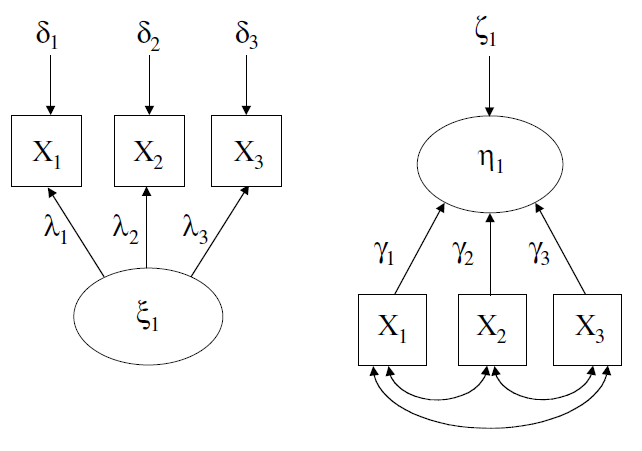
\includegraphics[scale=0.5]{chunks/borsboom}
\par\end{centering}

\caption{\label{fig:dag}(left) A reflexive model where the latent variable $\xi_{1}$ causes the observed $X_{i}$s. (right) A formative model where $\eta_{1}$ is defined in terms of the $X_{i}$s. This figure is taken from \cite[p. 61]{Borsboom2005-iq}.}
\end{figure}

When we have a psychometric model such as the one-factor model, we want to estimate the latent $Z$. Disregarding potential covariates $X$, an estimator of $Z$ must be based on the vector of observed variables $Y$ only. That is, $\hat{Z}=\phi(X)$, a function of the observed variables $X$. For generalized item response models, the maximum likelihood estimator of $Z$ or its posterior mean are common estimators of $Z$. These quantities are only defined when we make parametric assumptions about all random variables involved. But the linear one-factor model is a semi-parametric model, and the maximum likelihood estimator of $Z$ need not exists. The most widely used estimator of $Z$ in psychology is the \emph{sum
score}, $\hat{Z}=\sum_{i=1}^{k}X_{i}$, and the mean squared error-optimal linear combination $\hat{Z}=\sum_{i=1}^{k}v_{i}X_{i}$ is popular too. Both of these make sense mainly in the linear one-factor model. 

The three fundamental questions of psychometrics are:
\begin{enumerate}
\item \textbf{Model fit}. Is the model a good approximation to reality? Are the structural and parametric assumptions defensible? Model fit in structural equation modelling is usually evaluation through model fit indices, for instance $\chi^{2}$-tests. \parencite[Chapter 15]{Mulaik2009-gc}.
\item \textbf{Reliability}. Is $\hat{Z}$ a good estimator of $Z$, assuming the model is correct? If so, the estimator is reliable. In the linear one-factor model, the reliability is most often measured by calculating coefficient alpha \parencite{Cronbach1951-in}, a statistic related to the squared correlation $\Cor^{2}(Z,\hat{Z})$. between $Z$ and $\hat{Z}$ when $\hat{Z}$ is a sum-score.
\item \textbf{Validity}. Is $Z$ what we want it to be? Even if the model is correct, $Z$ might be something else than what we would like it to be. For instance, the five questions of Table \ref{tab:IPIP} should be related to the personality trait agreeableness. But is true? Maybe they measure some other psychological trait, such as irritability, intelligence, or even a physical trait such as height. Assuming personality traits such agreeableness exists, which not every psychometrician agrees with, there are some methods to check this. The techniques are often extrastatistical, and the application of them is called \emph{validation}. \parencite[Chapter 6]{Borsboom2005-iq}
\end{enumerate}